\section{Problems Encountered}
\label{sec:problems}
The development of this algorithm has encountered a number of important problems that affected its progress. This section will emphasise the most influential such issues and, if known, suggest a solution for resolving them.

To begin with, some edge-cases remained unaddressed. For example, Figure \ref{fig:edge} shows a frequently appearing such edge-case: the blue guard is stuck on the vertex because its movement direction cannot be projected inside the polygon. So, it cannot move downwards and is instead stuck on the vertex.

\begin{figure}[h!]
    \centering
    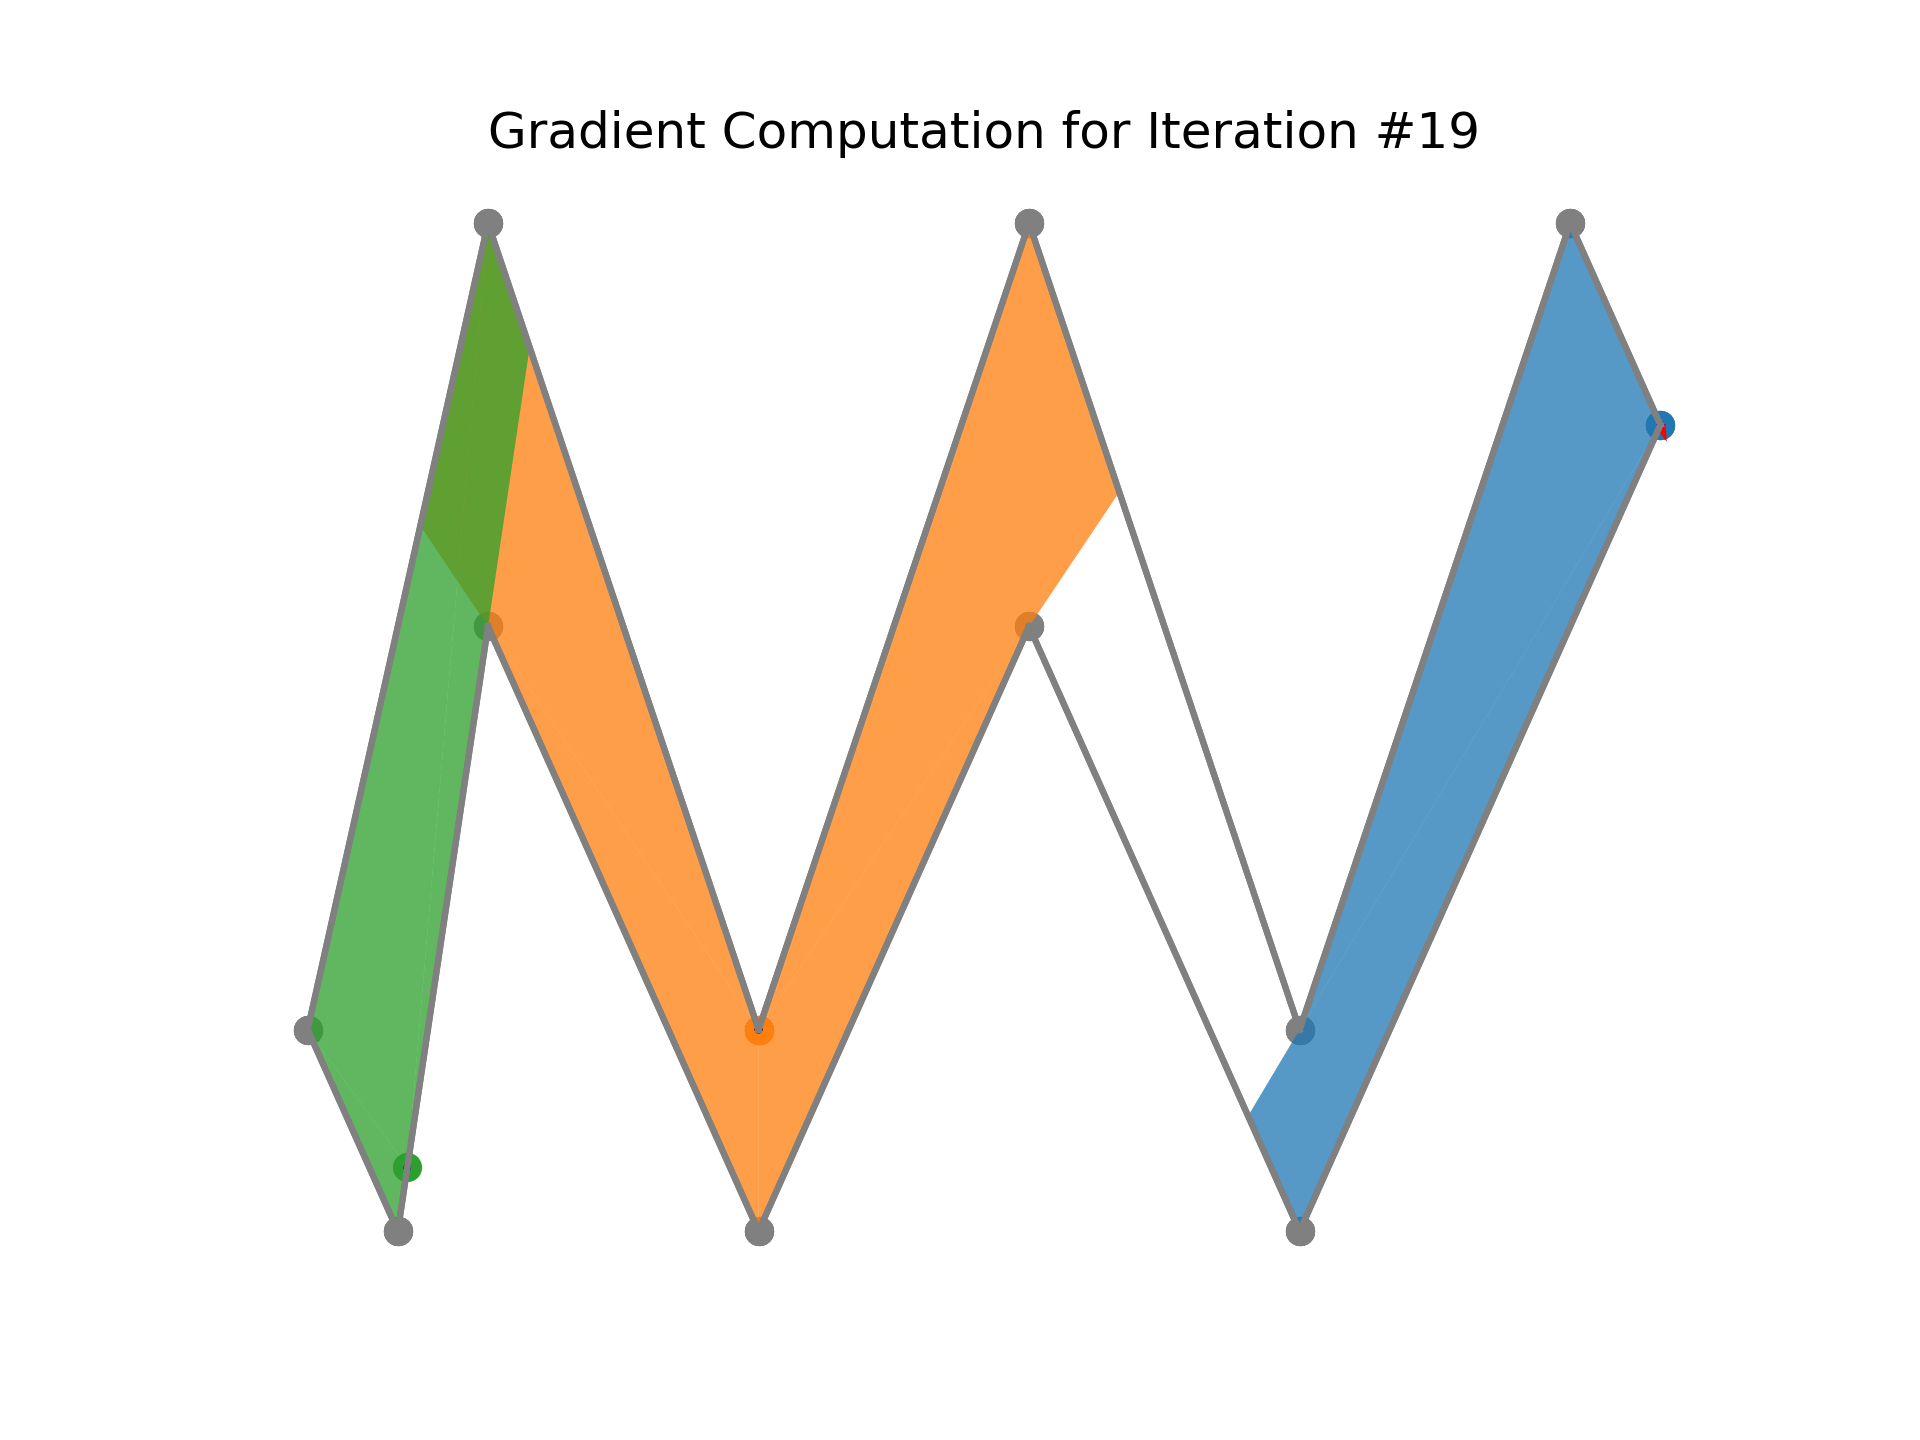
\includegraphics[width = 0.6\textwidth]{experiments/edge_case.png}
    \caption{Edge-case for when the blue guard cannot move because its movement direction cannot be projected towards the inside the polygon.}
    \label{fig:edge}
\end{figure}

Moreover, numerous issues were posed by the CGAL library itself. These problems mainly related to the library's non-detailed errors and brief documentation. Having to reverse engineer and delve into the source-code of CGAL slowed down the debugging process. Because some errors were not explicit at all, some crashes remained unsolved (for example, the program crashes for certain starting positions for different polygons). 

Some issues were posed by converting between CGAL's number types and the native C ++ types (\texttt{double}). This was necessary for speeding up the computations. Using only CGAL's types resulted in program runs longer than five minutes even for the smallest test cases. Approximation to \texttt{double}s allows us to reduce this time to near-instant results for the smallest test cases. Nonetheless, such conversion resulted in approximation errors. For instance, some guards ``close enough'' to reflex vertices were wrongly considered to be on the reflex vertex. Conversely, comparing point coordinates would not always work. Sometimes guards with the same coordinates would not be considered to be the same.

Additionally, we were especially interested in the irrational guards polygon \cite{abrahamsen2021art}. However, our program can only solve the irrational guards polygon if the guards are already very close to the optimum. For other starting positions, the program crashes with a mysterious CGAL error. Because of the vagueness of the error and the time constraints of the thesis, we could not fix this issue.

Lastly, we also wanted to test the program on polygons from the APGlib library \cite{art-gallery-instances-page}. The APGlib library offers an extensive testbed for polygons. Unfortunately, the same type of mysterious error happened with APGlib polygons with 20 vertices. Interestingly, the program only got stuck in a local minimum for one of the polygons with 20 vertices (polygon 3). Nonetheless, the fact that we could not address the CGAL error in this thesis' time constraints was quite dissatisfying.

Another problem worth mentioning is scalability. The program does not scale. As mentioned in Section \ref{sec:experiments}, for comb polygons with more than 6 teeth, the waiting time already exceeds an hour to finish. We believe that this waiting time is inadequate for the size and number of guards of the polygon.
Some of the largest bottlenecks that work against scalability are the visibility area and the Hidden Gradient computations. Currently, the visibility area of each guard is updated at every iteration. We are using the Triangular Expansion Visibility \cite{DBLP:journals/corr/BungiuHHHK14} which runs in $O(g)$ time, with $g$ the number of guards. Thus, the visibility computation per iteration runs in $O(g^2)$ time. 
In terms of the Hidden Gradient computation, each guard has its gradient recomputed at most $g$ times. This happens in the case when only one guard out of the $g$ guards has a non-zero gradient, and thus it gets removed from the set. The remaining $g - 1$ guards have their gradient recomputed. Again, in the worst case only one guard has a non-zero gradient. Thus, a guard gets its gradient recomputed in $O(g^2)$ time.
Other poorly scalable parts of the algorithm are based on the number of reflex vertices. The gradient computation depends on the number of reflex vertices $r$. If $r >> g$, then the algorithm will perform poorly for polygons with significantly fewer guards than reflex vertices.

For these reasons, the algorithm is sensitive to the heuristics used, the shape of the polygons and the values of the hyperparameters. In the Section \ref{sec:experiments} we have mentioned some shapes of polygons that the algorithm can solve, and with which hyperparameters initial guard positions.
We believe that if these edge-cases and errors get solved, the program should perform correctly and with no crashes for any input polygons. We would still expect that the program would get stuck in local minima. However, it should be possible to escape them with case-specific hyperparameter tuning and heuristic choice.
% Some of the polygons the algorithm can solve under the tested circumstances include those mentioned in Section \ref{sec:experiments}. 





% - cryptic CGAL errors
% - can only work with simple polygons
% - except for the few test polygons (2 guards, random, comb), all the other testbeds (Simon's) don't work because the algorithm gets stuck/crashes
% - for bigger polygons (more guards) it becomes slow very fast (unfeasible)
% - initial guard placement
